\section{Sanctuary Preparation and Furnishings}
Quiet, accurate preparation in the sacristy allows the sacred liturgy to unfold without hurry or confusion. The General Instruction of the Roman Missal (nos. 105, 117--119, 304--349) entrusts the sacristan with arranging the altar cloths, credence table, sacred vessels, folded linens, marked liturgical books, candles, incense, and seasonal vestments before the procession begins, and with guarding the reverent post-Mass care of altar linens and vessels. Every plate below pairs visual identification with the exact preparation standards of the 2008 Latin and 2011 United States Roman Missal.

\PCDPlateHeader{Plate I --- The Postconciliar Roman Sanctuary}{Not to common scale (architectural perspective)}
\ifdefined\TriptychPrintEdition
\begin{center}
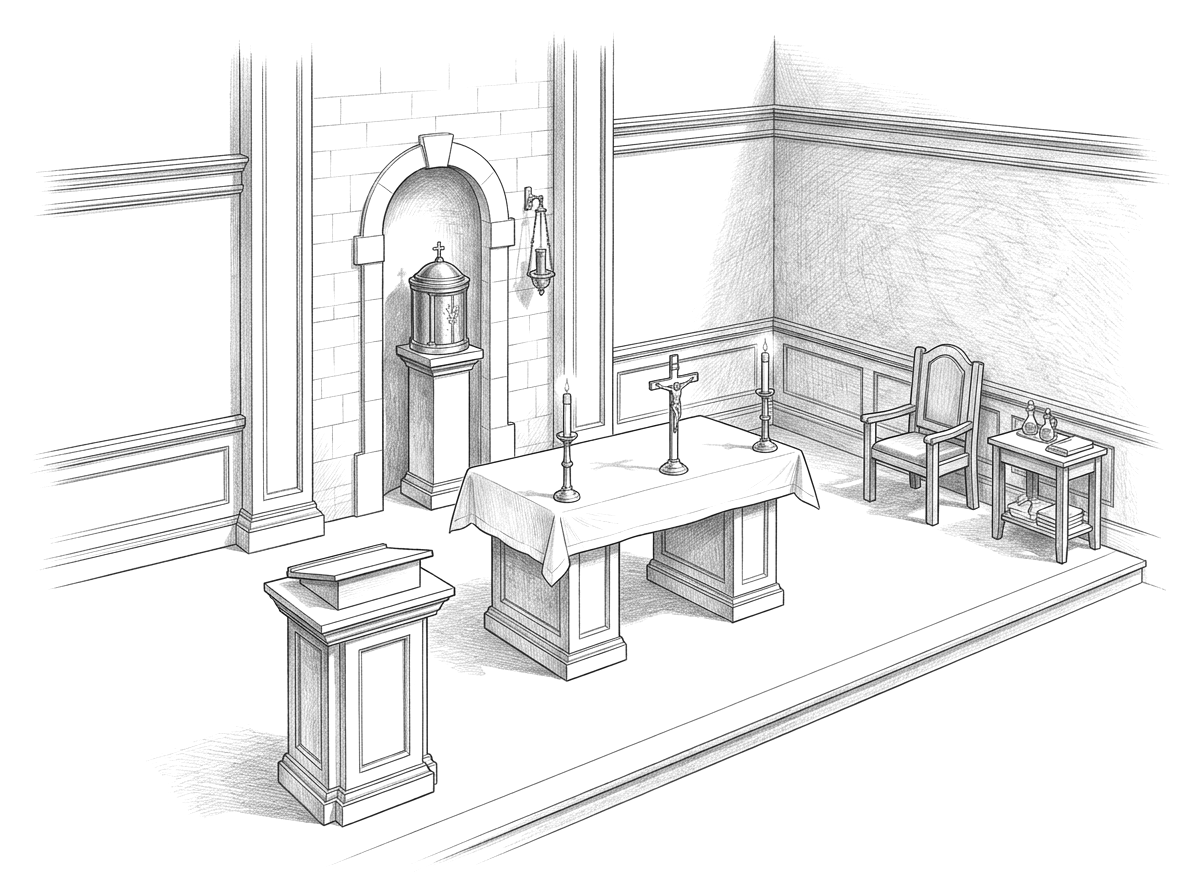
\includegraphics[width=0.96\linewidth,height=4.25in,keepaspectratio]{liturgy/roman-rite/postconciliar/2008-latin-2011-us-english/reference/roman-sanctuary-dictionary/shared/artwork/graphite/pc-art-01-sanctuary-composition.png}
\end{center}
\PCDPositionKey{Center: freestanding Altar with white Altar Cloth, two Altar Candles, and Altar Cross with corpus; foreground left: stationary Ambo; rear recessed niche: solid locked Tabernacle with hanging Sanctuary Lamp; rear right: Presidential Chair beside Credence Table holding cruets and linens.}
\else
\textbf{Visual Plate Summary (Plate I --- The Postconciliar Roman Sanctuary, Not to common scale (architectural perspective)):} Full architectural monochrome graphite perspective of a postconciliar Roman Catholic sanctuary showing the spatial coordination of freestanding stone altar dressed in white cloth with two candles and crucifix, permanent stone ambo in left foreground, wooden presidential chair and credence table with glass cruets and folded linens on the right, and a solid architectural tabernacle on a pillar inside a recessed arched niche with a hanging sanctuary lamp beside it. No altar cards, gradines, or rail appear.

\textbf{Reading order and object placement:} Center: freestanding Altar with white Altar Cloth, two Altar Candles, and Altar Cross with corpus; foreground left: stationary Ambo; rear recessed niche: solid locked Tabernacle with hanging Sanctuary Lamp; rear right: Presidential Chair beside Credence Table holding cruets and linens.
\fi

\subsection*{Monochrome Key for Liturgical Vestment Colors}
In monochrome graphite plates, vestment and textile colors appointed in the General Instruction of the Roman Missal (no.~346, with United States adaptations) are named in words and keyed below rather than encoded by tint alone.

\ifdefined\TriptychPrintEdition
{\footnotesize\begin{longtable}{>{\raggedright\arraybackslash}p{0.14\linewidth}>{\raggedright\arraybackslash}p{0.27\linewidth}>{\raggedright\arraybackslash}p{0.52\linewidth}}
\toprule
\textbf{Color} & \textbf{Monochrome key} & \textbf{Appointed occasions (US 2011 GIRM 346)} \\
\midrule
\endhead
\textbf{White} & \tikz[baseline=-0.5ex]{\draw[black,line width=0.5pt,fill=white] (0,0) rectangle (0.34cm,0.22cm);}\ Open white box (unshaded) & Easter Time, Christmas Time, celebrations of the Lord (except Passion), Blessed Virgin Mary, Angels, non-martyr Saints, All Saints, St. John the Baptist, St. John the Evangelist, Chair of St. Peter, Conversion of St. Paul; also permitted in the United States for funeral Masses (US GIRM 346e). \\
\textbf{Red} & \tikz[baseline=-0.5ex]{\draw[black,line width=0.5pt] (0,0) rectangle (0.34cm,0.22cm); \draw[black,line width=0.35pt] (0.06cm,0)--(0.06cm,0.22cm) (0.12cm,0)--(0.12cm,0.22cm) (0.18cm,0)--(0.18cm,0.22cm) (0.24cm,0)--(0.24cm,0.22cm) (0.29cm,0)--(0.29cm,0.22cm);}\ Vertical parallel rule & Palm Sunday of the Passion of the Lord, Good Friday, Pentecost Sunday, celebrations of the Passion of the Lord, birthdays (martyrdoms) of Apostles and Evangelists, and celebrations of Martyr Saints (GIRM 346b). \\
\textbf{Green} & \tikz[baseline=-0.5ex]{\draw[black,line width=0.5pt] (0,0) rectangle (0.34cm,0.22cm); \draw[black,line width=0.35pt] (0,0.12cm)--(0.10cm,0.22cm) (0,0.02cm)--(0.20cm,0.22cm) (0.08cm,0)--(0.30cm,0.22cm) (0.18cm,0)--(0.34cm,0.16cm) (0.28cm,0)--(0.34cm,0.06cm);}\ Diagonal rising hatch & Offices and Masses of Ordinary Time (GIRM 346c). \\
\textbf{Violet} & \tikz[baseline=-0.5ex]{\draw[black,line width=0.5pt] (0,0) rectangle (0.34cm,0.22cm); \draw[black,line width=0.3pt] (0,0.11cm)--(0.11cm,0.22cm) (0,0)--(0.22cm,0.22cm) (0.11cm,0)--(0.33cm,0.22cm) (0.22cm,0)--(0.34cm,0.12cm) (0,0.11cm)--(0.11cm,0) (0,0.22cm)--(0.22cm,0) (0.11cm,0.22cm)--(0.33cm,0) (0.22cm,0.22cm)--(0.34cm,0.10cm);}\ Cross-hatched grid & Advent and Lent; also lawful for Offices and Masses for the Dead (GIRM 346d). \\
\textbf{Black} & \tikz[baseline=-0.5ex]{\draw[black,line width=0.5pt,fill=black] (0,0) rectangle (0.34cm,0.22cm);}\ Solid black fill & Permitted where customary (including in the United States) for Masses for the Dead (US GIRM 346e). \\
\textbf{Rose} & \tikz[baseline=-0.5ex]{\draw[black,line width=0.5pt] (0,0) rectangle (0.34cm,0.22cm); \fill[black] (0.06cm,0.055cm) circle (0.4pt) (0.13cm,0.055cm) circle (0.4pt) (0.20cm,0.055cm) circle (0.4pt) (0.27cm,0.055cm) circle (0.4pt) (0.095cm,0.11cm) circle (0.4pt) (0.165cm,0.11cm) circle (0.4pt) (0.235cm,0.11cm) circle (0.4pt) (0.06cm,0.165cm) circle (0.4pt) (0.13cm,0.165cm) circle (0.4pt) (0.20cm,0.165cm) circle (0.4pt) (0.27cm,0.165cm) circle (0.4pt);}\ Fine stippled dots & Permitted where customary on Gaudete Sunday (Third Sunday of Advent) and Laetare Sunday (Fourth Sunday of Lent) (GIRM 346f). \\
\textbf{Gold or Silver} & \tikz[baseline=-0.5ex]{\draw[black,line width=0.6pt] (0,0) rectangle (0.34cm,0.22cm); \draw[black,line width=0.3pt] (0.04cm,0.04cm) rectangle (0.30cm,0.18cm);}\ Double-bordered festive frame & Festive vestments may be worn on more solemn occasions even if not of the color of the day (GIRM 346g); in the United States, gold- or silver-colored vestments are permitted on more solemn occasions (US GIRM 346h). \\
\bottomrule
\end{longtable}}
\else
{\footnotesize\begin{longtable}{>{\raggedright\arraybackslash}p{0.14\linewidth}>{\raggedright\arraybackslash}p{0.25\linewidth}>{\raggedright\arraybackslash}p{0.54\linewidth}}
\toprule
\textbf{Color} & \textbf{Print pattern key} & \textbf{Appointed occasions (US 2011 GIRM 346)} \\
\midrule
\endhead
\textbf{White} & Open white box (unshaded) & Easter Time, Christmas Time, celebrations of the Lord (except Passion), Blessed Virgin Mary, Angels, non-martyr Saints, All Saints, St. John the Baptist, St. John the Evangelist, Chair of St. Peter, Conversion of St. Paul; also permitted in the United States for funeral Masses (US GIRM 346e). \\
\textbf{Red} & Vertical parallel rule & Palm Sunday of the Passion of the Lord, Good Friday, Pentecost Sunday, celebrations of the Passion of the Lord, birthdays (martyrdoms) of Apostles and Evangelists, and celebrations of Martyr Saints (GIRM 346b). \\
\textbf{Green} & Diagonal rising hatch & Offices and Masses of Ordinary Time (GIRM 346c). \\
\textbf{Violet} & Cross-hatched grid & Advent and Lent; also lawful for Offices and Masses for the Dead (GIRM 346d). \\
\textbf{Black} & Solid black fill & Permitted where customary (including in the United States) for Masses for the Dead (US GIRM 346e). \\
\textbf{Rose} & Fine stippled dots & Permitted where customary on Gaudete Sunday (Third Sunday of Advent) and Laetare Sunday (Fourth Sunday of Lent) (GIRM 346f). \\
\textbf{Gold or Silver} & Double-bordered festive frame & Festive vestments may be worn on more solemn occasions even if not of the color of the day (GIRM 346g); in the United States, gold- or silver-colored vestments are permitted on more solemn occasions (US GIRM 346h). \\
\bottomrule
\end{longtable}}
\fi

\clearpage
\PCDPlateHeader{Plate II --- Principal Sanctuary Furnishings}{Not to common scale}
\ifdefined\TriptychPrintEdition
\begin{center}
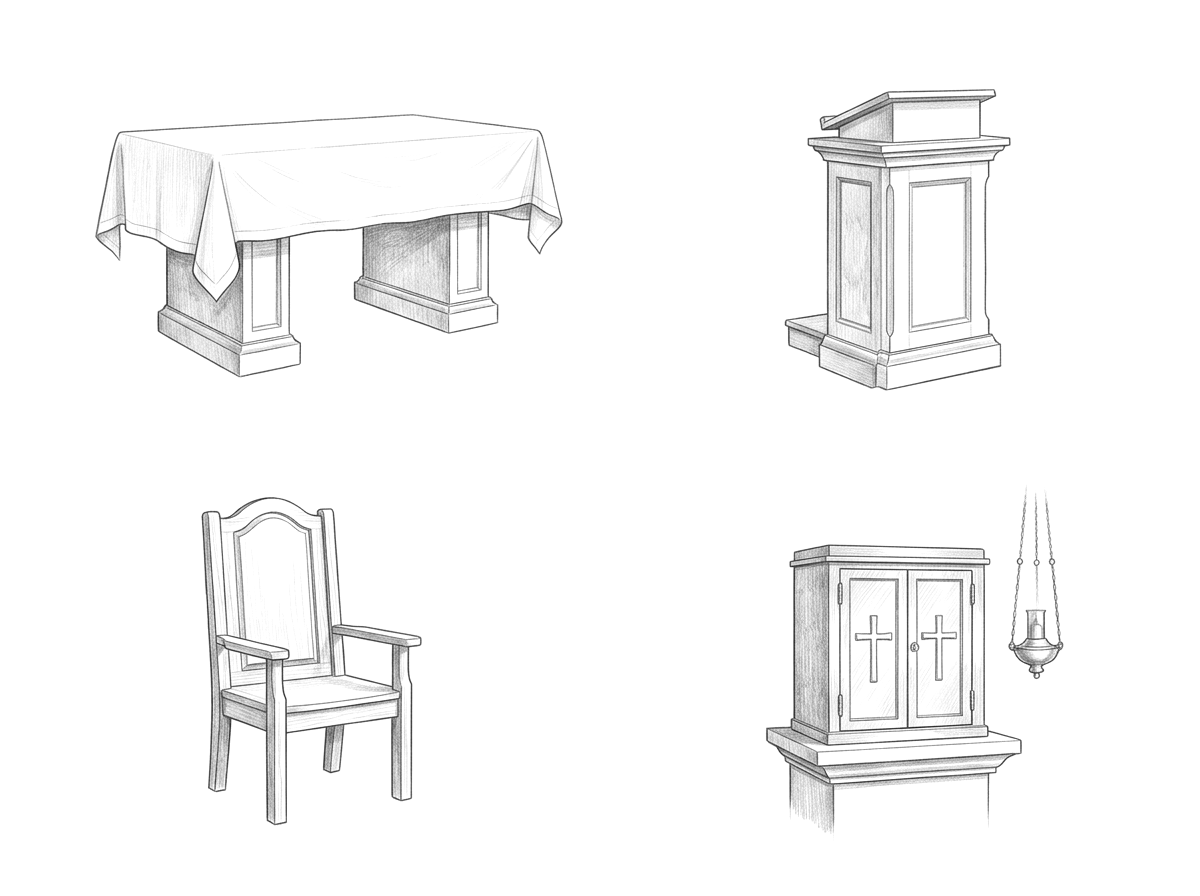
\includegraphics[width=0.92\linewidth,height=3.55in,keepaspectratio]{liturgy/roman-rite/postconciliar/2008-latin-2011-us-english/reference/roman-sanctuary-dictionary/shared/artwork/graphite/pc-art-02-altar-ambo-chair.png}
\end{center}
\PCDPositionKey{Top left: freestanding Altar covered with white linen cloth; top right: stationary stone Ambo with sloped desk and step; bottom left: dignified wooden Presidential Chair; bottom right: locked double-door Tabernacle on stone pedestal beside suspended oil Sanctuary Lamp.}
\else
\textbf{Visual Plate Summary (Plate II --- Principal Sanctuary Furnishings, Not to common scale):} Four-subject monochrome graphite architectural study comparing the principal sanctuary furnishings: top left, a freestanding carved stone altar dressed in a white linen altar cloth; top right, a permanent paneled stone ambo with angled book rest and rear step; bottom left, a stately wooden presidential chair with armrests; bottom right, a solid locked double-door metal tabernacle on a stone pedestal with a suspended sanctuary lamp burning beside it.

\textbf{Reading order and object placement:} Top left: freestanding Altar covered with white linen cloth; top right: stationary stone Ambo with sloped desk and step; bottom left: dignified wooden Presidential Chair; bottom right: locked double-door Tabernacle on stone pedestal beside suspended oil Sanctuary Lamp.
\fi

\label{pc-obj-altar}
\PCDEntryHead{Altar}{Altare}{required}{N01}
\PCDField{Also called}{Altar Table; Mensa; \textit{Mensa Domini}; \textit{Altare fixum}; \textit{Altare mobile}}
Ensure the mensa is clean, level, and dressed with at least one smoothly pressed white linen cloth proportioned to the altar's shape (GIRM 117, 304); where United States festive under-cloths are used (US GIRM 304), verify that the uppermost cloth remains white. Before Mass begins, keep the mensa completely bare of cruets, Missal stands, spare bulletins, and loose papers so that only the Book of the Gospels rests there during the Liturgy of the Word (GIRM 306). Inspect the mensa after Mass for wax drips and confirm that any Precious Blood spill has been tended exclusively by the priest or deacon (GIRM 280).

\PCDField{Plate position and norm}{Top left (Plate II); center (Plate I) (Universal Roman law)}
\PCDField{Placement and use}{Universal Roman law recommends a single fixed altar in newly built churches, set apart from the rear wall so ministers may walk around it and celebrate Mass facing the people wherever possible (GIRM 299, 303), while the Holy See clarified on 25 September 2000 (Prot. N. 2036/00/L) that this expresses pastoral desirability rather than a juridical ban on historical wall-attached altars or celebration facing the apse. A fixed altar is solemnly dedicated by the bishop (GIRM 300; CIC can. 1235), with relics of saints fittingly placed beneath it rather than recessed into the mensa (GIRM 302). From the start of Mass until the Preparation of the Gifts, only the Book of the Gospels rests upon the dressed mensa; during the Liturgy of the Eucharist, only the corporal, sacred vessels, Roman Missal, and necessary items appear there (GIRM 306).}
\PCDField{United States norm}{In the Dioceses of the United States of America, the Bishops' Conference adaptation to GIRM 301 permits a fixed altar table to be crafted from dignified, solid, well-worked wood rather than natural stone, provided the structure remains permanently immovable; United States GIRM 304 likewise allows festive colored cloths beneath the required white uppermost cloth.}
\PCDField{Prepared and handled by}{Prepares: Sacristan, Deacon, Instituted acolyte, Altar server. Ministers in use: Bishop, Priest, Deacon.}
\PCDSafety{Keep the altar table clear of spare papers, cruets, and extraneous items (GIRM 306), guard against candle flames and dripping wax near the white cloth, and notify the priest or deacon immediately if any Precious Blood is spilled---never attempt to blot or wash a spill yourself (GIRM 280).}
\PCDField{Distinguish from}{Credence Table}
\PCDEntryRule

\label{pc-obj-ambo}
\PCDEntryHead{Ambo}{Ambo}{required}{N02}
\PCDField{Also called}{Lectern of the Word; \textit{Lectrinum}}
Before Mass, place the Lectionary---never a disposable booklet---neatly upon the ambo desk and open it to the appointed first reading (GIRM 118b, 349). Confirm that the desk is clear of parish announcements, music folders, and stray papers, that any lighting or microphone works cleanly without obstructing the Book of the Gospels, and that a separate lectern stands outside the ambo's focal area for a commentator or song leader when needed (GIRM 309).

\PCDField{Plate position and norm}{Top right (Plate II); left foreground (Plate I) (Universal Roman law)}
\PCDField{Placement and use}{Universal Roman law prescribes a permanent, stationary ambo---never a lightweight movable lectern---positioned so that the attention of the faithful turns naturally toward it during the Liturgy of the Word and ministers can be clearly seen and heard (GIRM 309; Ordo lectionum Missae 32--34). Only the Scripture readings, the Responsorial Psalm, and the Easter Proclamation (Exsultet) are proclaimed from the ambo, together with the homily and the intentions of the Universal Prayer; parish announcements, commentary, and the leading of general singing belong at a separate stand elsewhere.}
\PCDField{Prepared and handled by}{Prepares: Sacristan, Instituted lector, Altar server. Ministers in use: Bishop, Priest, Deacon, Instituted lector.}
\PCDSafety{Watch the rear step of the ambo when moving into place with lighted Gospel candles or a smoking thurible, keeping flames well clear of the microphone, Lectionary pages, and ministers' vestments.}
\PCDField{Distinguish from}{Missal Stand}
\PCDEntryRule

\label{pc-obj-presidential-chair}
\PCDEntryHead{Presidential Chair}{Sedes sacerdotis celebrantis}{required}{N03}
\PCDField{Also called}{Chair for the Priest Celebrant; Presider's Chair; \textit{Sedes}}
Before Mass, set the marked Roman Missal---or the official United States Excerpts from the Roman Missal (Book of the Chair)---along with a hymnal or worship aid neatly on a small stand beside the presidential chair (GIRM 118a). Verify that the chair sits cleanly in its appointed place with clear floor space in front for the book-bearer, and keep loose notes, water bottles, or clutter out of sight.

\PCDField{Plate position and norm}{Bottom left (Plate II); rear right (Plate I) (Universal Roman law)}
\PCDField{Placement and use}{Under universal Roman law, the chair is best set at the head of the sanctuary facing the congregation unless architectural distance or a centrally placed tabernacle behind the altar makes another clear position more suitable (GIRM 310). From this seat the priest conducts the Introductory Rites (including the Collect), listens to the Scripture readings and may preach the homily, leads the Universal Prayer, and concludes Mass with the Prayer after Communion and dismissal (GIRM 124, 127--130, 165--167). The Roman Missal---or, in the United States, the lighter Book of the Chair---and any needed hymnal are prepared beside it (GIRM 118a). In a cathedral church, the diocesan bishop presides from his permanent cathedra rather than a presbyteral chair (Caeremoniale Episcoporum 1984).}
\PCDField{Prepared and handled by}{Prepares: Sacristan, Altar server. Ministers in use: Priest, Bishop.}
\PCDEntryRule

\label{pc-obj-credence-table}
\PCDEntryHead{Credence Table}{Abacus}{required}{N04}
\PCDField{Also called}{Side Table; Credence; \textit{Credentia}; \textit{Mensa credentiae}}
Cover the credence table with a clean white linen cloth and verify every item listed in GIRM 118c: blessed principal chalice with folded corporal, purificator, optional pall and chalice veil; paten and any extra ciboria or Communion chalices with one purificator apiece; stoppered wine and water cruets on their tray; lavabo pitcher, basin, and finger towel; Communion-plate; and aspersorium when the sprinkling rite is scheduled. Leave open space on the tabletop so the priest, deacon, or instituted acolyte can purify vessels cleanly on a corporal after Communion or after Mass (GIRM 279).

\PCDField{Plate position and norm}{See Plate I, far right beside the presidential chair (Universal Roman law)}
\PCDField{Placement and use}{GIRM 118c appoints the credence table (abacus) as the preparation station for every Mass with a congregation, holding the chalice, folded corporal, purificator, optional pall and chalice veil, paten, ciboria, bread and wine cruets (unless carried in the Procession of Gifts), vessel of blessed water for the Sunday sprinkling rite, Communion-plate, and lavabo pitcher, basin, and towel. Keeping these items on the credence table preserves an uncluttered altar mensa until the Preparation of the Gifts (GIRM 139, 306). After Communion or immediately after Mass, sacred vessels may also be purified at the credence table by a priest, deacon, or instituted acolyte (GIRM 279).}
\PCDField{Prepared and handled by}{Prepares: Sacristan, Instituted acolyte, Altar server. Ministers in use: Priest, Deacon, Instituted acolyte.}
\PCDSafety{After Communion, never purify sacred vessels at the credence table and never disturb unpurified vessels left suitably covered upon a corporal there; purification belongs strictly to the priest, deacon, or instituted acolyte (GIRM 279; Redemptionis Sacramentum 119; USCCB Norms 53).}
\PCDField{Distinguish from}{Altar}
\PCDEntryRule

\label{pc-obj-tabernacle}
\PCDEntryHead{Tabernacle}{Tabernaculum}{required}{N05}
\PCDField{Also called}{Eucharistic Tabernacle}
Keep the exterior of the tabernacle, its stone pedestal, and its surrounding prayer area spotless, while respecting the canonical security of the key under the pastor's responsibility (CIC can. 938 §5). Never leave the key resting unattended in the lock or on an open sacristy hook. Confirm that a clean linen corporal lines the interior floor (placed by clergy or an authorized minister), ensure that the continuous oil or wax sanctuary lamp burns beside it whenever hosts are reserved (GIRM 316), and prepare to leave the tabernacle empty and open on Good Friday until the Easter Vigil.

\PCDField{Plate position and norm}{Bottom right (Plate II); recessed rear niche (Plate I) (Universal Roman law)}
\PCDField{Placement and use}{Universal Roman law requires ordinarily one tabernacle in a church or oratory, immovable, crafted of solid opaque material, securely locked against danger of profanation, and blessed before liturgical use (GIRM 314; CIC can. 938; Redemptionis Sacramentum 130). Because the sign of Mass is clearer when the tabernacle does not stand upon the altar of celebration, universal law (GIRM 315) entrusts the Diocesan Bishop to place it either in the sanctuary apart from the altar of celebration---not excluding a former high altar no longer used for Mass---or in a distinct chapel suitable for private adoration that is organically connected to the church and readily visible to the faithful. The pastor or rector must diligently safeguard the tabernacle key (CIC can. 938 §5).}
\PCDField{Prepared and handled by}{Prepares: Priest, Deacon. Ministers in use: Bishop, Priest, Deacon.}
\PCDSafety{Never open the tabernacle, touch the tabernacle key, or retrieve or repose the Blessed Sacrament. Key custody belongs strictly to the pastor or rector (CIC can. 938 §5). Genuflect on the right knee before the tabernacle outside Mass and at the beginning and end of Mass when it stands in the sanctuary (GIRM 274).}
\PCDEntryRule

\label{pc-obj-sanctuary-lamp}
\PCDEntryHead{Sanctuary Lamp}{Lampas peculiaris}{required}{N06}
\PCDField{Also called}{Tabernacle Lamp; Presence Lamp; \textit{Lampas sanctuarii}; \textit{Lucerna}}
Inspect the sanctuary lamp daily so that a living oil or wax flame---never a substitute electric light---shines without interruption whenever the Eucharist is reserved (GIRM 316; CIC can. 940). Replace seven-day or fourteen-day beeswax cylinders or refill oil reservoirs before the flame burns low, letting heated glass cool before handling and keeping spare wicks and globes clean. Extinguish and remove the flame only when the tabernacle has been completely emptied, as on Good Friday.

\PCDField{Plate position and norm}{Suspended beside the tabernacle at bottom right (Plate II) and in the rear niche (Plate I) (Universal Roman law)}
\PCDField{Placement and use}{Universal Roman law and canon law require a special lamp, nourished by oil or wax rather than an electric bulb, to shine permanently day and night beside every tabernacle in which the Most Holy Eucharist is reserved (GIRM 316; CIC can. 940). It is extinguished only when the tabernacle is completely emptied of the Blessed Sacrament, notably from the Mass of the Lord's Supper on Holy Thursday evening until reservation resumes at the Easter Vigil.}
\PCDField{Prepared and handled by}{Prepares: Sacristan. Ministers in use: Priest, Sacristan.}
\PCDSafety{Never extinguish, move, or adjust the sanctuary lamp during Mass, and never extinguish it while the Blessed Sacrament remains reserved in the tabernacle. If assisting the sacristan outside Mass to replace a sanctuary candle or oil vessel, allow hot glass and oil to cool safely, guard against open flame, and never open the tabernacle.}
\PCDField{Distinguish from}{Altar Candles}
\PCDEntryRule

\label{pc-obj-baptismal-font}
\PCDEntryHead{Baptismal Font}{Fons baptismalis}{required}{N07}
\PCDField{Also called}{Font; \textit{Fons baptismatis}}
Before every Baptism and especially before the Easter Vigil, scrub the font basin thoroughly and fill it with fresh, clean water (warmed gently when infants are baptized). Keep the removable domed cover clean and steady when lifted, stage clean linen towels, a pouring shell or pitcher, the baptismal candle, and the labeled Oil of Catechumens and Sacred Chrism nearby, and verify that any drained blessed water flows strictly into the sacrarium or clean earth.

\PCDField{Plate position and norm}{See Plate X, bottom right (Universal Roman law)}
\PCDField{Placement and use}{The baptismal font is governed by universal canon law (CIC can. 858 §1, requiring a font in every parish church), the Rite of Baptism for Children (General Introduction 25, 45--47), and the Easter Vigil rubrics of the Roman Missal. Local architecture places it either in a distinct baptistery or in a prominent, clearly visible area near the church entrance or sanctuary so the assembly can participate in Baptisms and process to the font at the Easter Vigil; its design accommodates clean flowing or poured water (and, where provided, immersion). Bishops, priests, and deacons are the ordinary ministers of Baptism (CIC can. 861 §1).}
\PCDField{Prepared and handled by}{Prepares: Sacristan, Deacon, Altar server. Ministers in use: Bishop, Priest, Deacon.}
\PCDSafety{Never empty blessed baptismal water into an ordinary sink or sewer drain; blessed water must be poured reverently into the sacrarium or directly into clean earth. Wipe any splashed water from stone or tiled steps immediately to prevent slipping.}
\PCDField{Distinguish from}{Aspergillum and Aspersorium}
\PCDEntryRule
